\documentclass{article}
\usepackage[utf8]{inputenc}
\usepackage{graphicx}

\begin{document}

\section{Presence and location}

\subsection{Objective and Functionality}
The presence and location is a set of two devices each with an ultrasonic sensor that determine user presence and location (left-right). Each of the sensors is responsible of sending collected data to their respective topic (sensor1/distance or sensor2/distance).

\subsection{Project Definition and Milestones}
The development of the presence and location system just involves establishing an MQTT connection with the broker to send the collected data from the ultrasonic sensors.

\subsection{Milestones Execution Order, Priority, and Dependencies}
\begin{enumerate}
    \item \textbf{Milestone 1: Establishing MQTT Communication}
       - \textit{Priority:} High. Fundamental for data transmission.
       - \textit{Dependencies:} Basic WiFi setup.
       - \textit{Execution Order:} First, as it is crucial for data reception.

    \item \textbf{Milestone 2: Send the collected that from the sensor}
       - \textit{Priority:} High. Essential for functionallity
       - \textit{Dependencies:} Successful MQTT setup.
       - \textit{Execution Order:} Second, building upon established communication.
\end{enumerate}

\subsection{Hardware Development}
The hardware setup for the location and presence comprises:
\begin{itemize}
    \item Two ESP-01 modules.
    \item Two ultrasonic sensor, one for each ESP-01 module.
\end{itemize}

\subsection{Software Implementation}
The software, written in arduino programming language, has the following key functionalities:
\begin{itemize}
    \item Connect to WiFi (and try to reconnect if needed).
    \item Establish MQTT connection.
    \item Measure and calculate distance using ultrasonic sensor pins.
    \item Send the resulting data to the corresponding topic (sensor1/distance or sensor2/distance)
\end{itemize}

\subsection{Interaction with Other Components}
The presence and distance system is based on an interaction between ESP01 modules and ultrasonic sensors to achieve effective communication of the user distance and presence to both the System Monitor (for displaying the data on the screen) and the RaspberryPi (for making it possible to predit who is the user).

\subsection{Testing}
Testing ensured accurate sensor data transmission via MQTT. An iterative approach was applied to refine the system's performance.

\subsection{Dedication Time}
Approximately 15 hours were dedicated to developing the System Monitor, mainly spent on finding out sensor malfunctioning given that the software implementation was simple and straightforward.

\subsection{User Story}
As a user approaches, the System Monitor recieves data about their presence, lighting up the LED bar and displaying their approximate location (left, right, or center) on the LCD screen, providing real-time feedback.

\subsection{Challenges and Solutions}
\begin{itemize}
    \item \textbf{Hardware Challenges:} Malfunctioning sensors which drove us crazy.
    \item \textbf{Software Challenges:} Processing sensor data accurately, since this cheap sensors can provide really confusing data.
\end{itemize}

\subsection{Hardware and Software Integration}
\begin{figure}[ht]
    \centering
    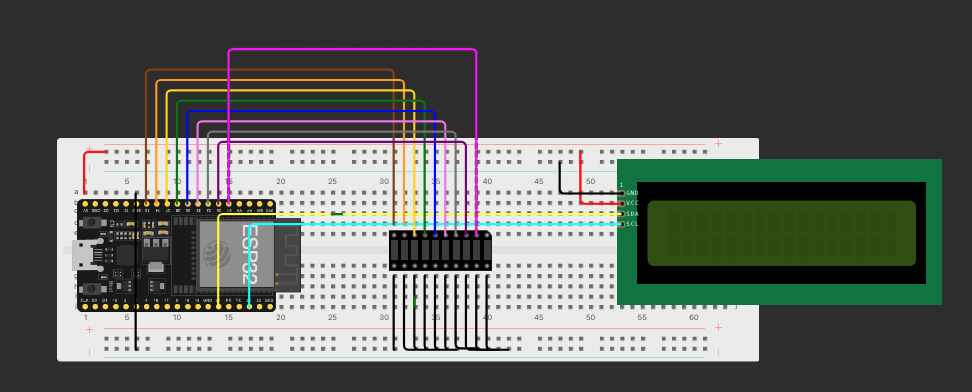
\includegraphics[width=0.8\textwidth]{../images/activity_monitor_scheme.png}
    \caption{ESP32 with LED bar and LCD display connected on a breadboard.}
    \label{fig:esp32_system_monitor}
\end{figure}

\subsection{Microcontroller Interaction Protocol}
The location and presence system involves a simple communication in one direction, basically the ESP01 have to send the collected data to their corresponding topics. The communication structure is the following:

\subsubsection{Communication Protocol}
The project utilizes the MQTT (Message Queuing Telemetry Transport) protocol, a lightweight and efficient messaging protocol ideal for IoT applications. This protocol is chosen for its low bandwidth usage and its ability to provide reliable communication over WiFi.

\subsubsection{WiFi Configuration}
Each microcontroller in the system is configured to connect to a WiFi network, enabling them to send data over the network. The network credentials (SSID and password) are programmed into the microcontrollers.

\subsubsection{Data Flow and Configuration}

\subsection{MQTT Tree Structure}
The MQTT protocol in the presence and location project uses a structured approach to manage the data flow. Below is the outline of the MQTT topics and their functions:

\subsubsection{MQTT Topics}
\begin{itemize}
    \item \textbf{sensor1/distance:} This topic is used by the first ESP-01 module. It publishes the distance data measured by its connected ultrasonic sensor.
    \item \textbf{sensor2/distance:} Similar to the first, this topic is for the second ESP-01 module.
\end{itemize}

\subsubsection{Data Organization and Utilization}
The data sent to these topics include numerical values representing the measured distances. 

\end{document}
